\documentclass[acmsmall,screen,nonacm]{acmart}
\setcopyright{none}
\raggedbottom

\usepackage{amsmath}
\usepackage{booktabs}
\usepackage{tabularx}
\usepackage{array}
\usepackage{tikz}
\usetikzlibrary{arrows.meta,positioning,fit}
\usepackage{enumitem}
\usepackage{microtype}

\newcolumntype{Y}{>{\raggedright\arraybackslash}X}
\newcommand{\BOne}{B1}
\newcommand{\BTwo}{B2}
\newcommand{\BThree}{B3}

\title{What a Resolving DOI Doesn't Tell You: An Error-Type Audit of Simple Citation Checkers}
\author{Bayyapu Vamshidhar Reddy}
\affiliation{\institution{Indian Institute of Information Technology Allahabad}\city{Prayagraj}\country{India}}

\keywords{citation verification, hallucinated references, bibliographic metadata, Crossref, false positives, evaluation}

\begin{document}
\begin{abstract}
Tools that check reference lists for hallucinated citations usually start with a simple question: does the DOI resolve? I tested what that question can and can't catch, and what happens when a checker goes further and compares the citation's title, authors, year and venue with the registry record. Three transparent, rule-based checkers were run on constructed citations built from Crossref records: a DOI-only control (\BOne{}), a field-matching checker (\BTwo{}) and a single-rule variant of it (\BThree{}). The data were a preregistered held-out set of 8 works and a random sample of 40 journal articles drawn under a logged protocol amendment, with eight citation variants per work. \BOne{} caught only the citations whose DOI doesn't exist (macro recall 0.20). Wrong years, wrong authors, borrowed DOIs and spliced titles all passed. \BTwo{} caught every constructed error (macro recall 1.00) with no false flags on the preregistered valid cases. That result is close to guaranteed, though, because the labels and the lookup share one registry. The more informative test used 87 \emph{legitimate} variants of real citations: first-author-only (``et al.'') lists, abbreviated journal names, dropped subtitles, print-versus-online year differences and PDF hyphenation breaks. \BTwo{} flagged 54\% of them, and each false flag traced back to one field rule. Changing only the author rule from a Jaccard threshold to set containment (\BThree{}) cut false flags to 19.5\% (paired source-clustered bootstrap difference $-0.39$ to $-0.29$) without losing recall. Re-scoring the same predictions under an identity-only definition of ``error'' dropped \BTwo{}'s precision from 1.00 to 0.60. Citation-checker accuracy can't be summarized without saying which errors are counted and which legitimate variations are expected. All code, frozen inputs and outputs are released.
\end{abstract}

\maketitle

\section{Introduction}
Fabricated references are no longer just a chatbot curiosity. Audits have found them in accepted papers at major machine-learning and security venues \citep{russinovich2026} and in hundreds of papers across ACL conferences \citep{sakai2026}, and commercial deep-research agents still produce citation URLs that point nowhere \citep{rao2026}. The obvious response is automated checking: take each reference, look it up in a bibliographic database, and flag what doesn't match.

My earlier literature review on citation fabrication ended with a gap the field itself acknowledges. We know a great deal about how often generators fabricate references, and very little about how accurate the checkers are. When I went back to the original papers, Russinovich et al.\ turned out to be explicit about this. Their checker's flags needed human review because many were false positives, caused by things like editors listed as co-authors, title fragments parsed as author names, real works not yet indexed, and preprint-versus-published drift \citep{russinovich2026}. They describe these causes but don't count them. Walters and Wilder make a related distinction on the generation side: a fabricated citation and an error in a real citation are different failures \citep{walters2023}.

This paper takes that gap at the scale a course project can handle honestly. I don't evaluate a published tool. Instead I build three deliberately simple, inspectable checkers and ask which kinds of citation error each one catches, and what each costs in false alarms on citations that are legitimately written differently from the registry. Simple checkers are worth studying because their failures can be traced to a single line of code, which a learned or LLM-based checker doesn't allow.

The study asks three questions:
\begin{description}[leftmargin=1.2em,itemsep=1pt]
\item[RQ1] Does checking metadata fields detect more constructed citation errors than checking that the DOI resolves?
\item[RQ2] Which error types and which legitimate citation variants cause misses or false flags, and which field rule is responsible?
\item[RQ3] How much does the definition of ``error'' change the measured accuracy of the same predictions?
\end{description}

\paragraph{What is and isn't new.} Controlled corruption of citations as a test bed isn't my idea. CiteCheck already evaluates retrieval-grounded checking on a controlled-corruption benchmark \citep{khajavi2026citecheck}, and Badalova and Mayr review what current reference-checking tools can and can't do \citep{badalova2026}. What this study adds is narrower: (i) a per-error-type audit of DOI-only and field-matching controls with abstention reported separately, (ii) a measured false-flag rate on five legitimate variant types, two of which (version drift and PDF extraction artifacts) correspond directly to false-positive causes described by Russinovich et al., (iii) a field ablation and a single-rule modification that explain where those false flags come from, and (iv) a demonstration that the label definition alone moves precision by 40 points. None of the numbers below estimate how often language models fabricate citations.

\section{Related Work}
\paragraph{Measuring fabrication.} Most of the evidence counts fabricated or erroneous references in generated text. Walters and Wilder examined citations generated by ChatGPT and reported fabricated citations separately from substantive errors in real ones, with very different rates for GPT-3.5 and GPT-4 \citep{walters2023}. Rao et al.\ audited URLs from commercial models and deep-research agents, finding that 3--13\% were hallucinated and 5--18\% did not resolve \citep{rao2026}. Sakai et al.\ traced hallucinated references through published ACL-venue papers \citep{sakai2026}. These studies measure \emph{generators}. Their checking procedures are part of the method, not the object of study.

\paragraph{Checking references.} Russinovich et al.\ check around 48{,}000 accepted papers from four venues against several bibliographic sources, escalating unresolved cases. They use a strict definition (no matching work, or a substantially wrong author list) and record but don't count venue or year drift \citep{russinovich2026}. CiteCheck combines retrieval with LLM verification and is evaluated on deliberately corrupted citations \citep{khajavi2026citecheck}. Agrawal et al.\ take another route and ask the generating model consistency questions about its own references \citep{agrawal2024}. A naming hazard is worth flagging: ``RefChecker'' also names an unrelated claim-level hallucination checker by Hu et al.\ \citep{hu2024refchecker}, which doesn't check bibliographies.

\paragraph{Where this study sits.} This is closest in spirit to CiteCheck's controlled corruption, but it uses no retrieval beyond a DOI lookup and no language model. In exchange, every decision is explainable by a single failed field, which makes the false-flag analysis possible.

\section{Study Design}
\subsection{Pipeline}
Fig.~\ref{fig:pipeline} summarizes the study. Every checker receives only the observed citation (DOI, title, author surnames, year, venue). The source identity, mutation category and labels are visible only to the scorer.

\begin{figure}[t]
\centering
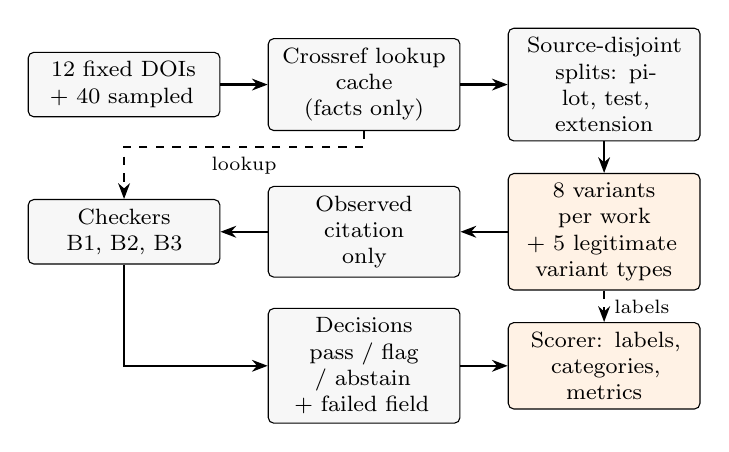
\begin{tikzpicture}[node distance=4mm and 6mm, every node/.style={font=\footnotesize, align=center},
  box/.style={draw, rounded corners=2pt, minimum height=8mm, text width=22mm, fill=gray!6},
  hid/.style={box, fill=orange!10}, arr/.style={-{Stealth[length=2mm]}, thick}]
\node[box] (doi) {12 fixed DOIs\\+ 40 sampled};
\node[box, right=of doi] (cache) {Crossref lookup\\cache (facts only)};
\node[box, right=of cache] (split) {Source-disjoint\\splits: pilot, test,\\extension};
\node[hid, below=of split] (mut) {8 variants per work\\+ 5 legitimate\\variant types};
\node[box, left=of mut] (obs) {Observed citation\\only};
\node[box, left=of obs] (chk) {Checkers\\\BOne{}, \BTwo{}, \BThree{}};
\node[hid, below=of mut] (score) {Scorer: labels,\\categories, metrics};
\node[box, left=of score] (out) {Decisions\\pass / flag / abstain\\+ failed field};
\draw[arr] (doi) -- (cache); \draw[arr] (cache) -- (split); \draw[arr] (split) -- (mut);
\draw[arr] (mut) -- (obs); \draw[arr] (obs) -- (chk); \draw[arr] (chk) |- (out);
\draw[arr] (out) -- (score); \draw[arr, dashed] (mut) -- node[right, font=\scriptsize]{labels} (score);
\draw[arr, dashed] (cache.south) -- ++(0,-2mm) -| node[pos=.25, below, font=\scriptsize]{lookup} (chk.north);
\end{tikzpicture}
\caption{Study pipeline. Shaded orange boxes hold information the checkers never see. The dashed line from the cache is the registry lookup that \BOne{}--\BThree{} share.}
\Description{Flow diagram: DOI list and random sample feed a Crossref cache, then source-disjoint splits, then citation variants. Checkers see only the observed citation; the scorer alone sees labels.}
\label{fig:pipeline}
\end{figure}

\subsection{Data}
\paragraph{Preregistered set.} Twelve DOIs were fixed in a protocol (version 1.0, frozen 2026-10-30) before any data were acquired. Their records were retrieved from the Crossref REST API \citep{crossrefapi}, shuffled with seed 20261030 and split by \emph{source work} into four pilot works and eight held-out test works. The pilot was used in an earlier phase to validate \BOne{}. The test works were not scored until the comparison reported here.

\paragraph{Extension set (amendment A1).} Eight works are too few for any interval estimate, as the frozen protocol itself noted. Before any held-out output existed, I logged an amendment that kept the original comparison unchanged and added a random extension set. A single call to Crossref's \texttt{sample} endpoint (journal articles only) returned 100 records. 91 met the eligibility rules (a title of at least three words, at least one named author, a year and a journal title), and the first 40 by DOI were frozen with a SHA-256 hash. The sample spans publication years 1921--2026, with a median of 2012. Ten of the 40 titles contain non-ASCII characters, and 17 of the 40 DOIs come from a single publisher prefix (10.1016). Because the \texttt{sample} endpoint cannot be replayed, the saved snapshot is the frozen artifact.

\paragraph{Constructed errors.} For every work, eight citations were generated (Table~\ref{tab:variants}). Donor works for wrong-DOI and Frankenstein cases come from the same split. Each split's source works are disjoint from every other split's, and the code rejects any case file that breaks this.

\begin{table}[t]
\caption{Citation variants. ``Any-error'' and ``identity-only'' are the two label definitions used for RQ3. Legitimate variants are always labelled valid and are scored separately.}
\label{tab:variants}
\footnotesize
\begin{tabularx}{\linewidth}{@{}l Y c c@{}}
\toprule
Variant & Construction & Any-error & Identity \\
\midrule
clean & Registry record as is & valid & valid \\
format variant & DOI as uppercase URL, title in capitals & valid & valid \\
missing DOI & DOI removed (checkers must abstain) & valid & valid \\
wrong year & Year $+7$ & error & valid \\
wrong author & Author list replaced by a non-author & error & error \\
wrong DOI & DOI of another real work in the split & error & valid \\
Frankenstein & Title of another real work in the split & error & error \\
synthetic unmatched & Non-existent DOI and title & error & error \\
\midrule
\multicolumn{4}{@{}l}{\emph{Legitimate variants (extension set only; applied when the record allows)}}\\
``et al.'' & First author only ($\geq 2$ authors; $n=30$) & \multicolumn{2}{c}{valid} \\
abbreviated venue & Crossref's own short journal title ($n=11$) & \multicolumn{2}{c}{valid} \\
subtitle dropped & Title cut at the first colon ($n=6$) & \multicolumn{2}{c}{valid} \\
print-year drift & Print year where it differs from the earliest year ($n=1$) & \multicolumn{2}{c}{valid} \\
hyphen break & Longest word split as in PDF extraction ($n=39$) & \multicolumn{2}{c}{valid} \\
\bottomrule
\end{tabularx}
\end{table}

The legitimate variants are the core of RQ2. Each imitates a way real reference lists differ from registry records without being wrong. Print-year drift and hyphen breaks correspond directly to causes Russinovich et al.\ describe (version drift and PDF extraction errors). The other three are ordinary citation conventions that I added because a field-matching checker is obviously exposed to them. All five are \emph{registry-derived approximations}: the abbreviations are Crossref's own short titles and the print years are Crossref's own print dates, not forms observed in real reference lists. Their counts reflect how many records allowed each variant, not how common each form is in practice.

\subsection{Checkers}
All three checkers normalize DOIs (prefix, URL and case) and look the DOI up in the same cache. A missing DOI produces an abstention, and a DOI with no Crossref record produces a flag. Network failures abort the run and are never counted as fabrications.
\begin{description}[leftmargin=1.2em,itemsep=1pt]
\item[\BOne{} DOI-only.] Passes any citation whose DOI resolves.
\item[\BTwo{} field matching.] Also requires title similarity $\geq 0.90$ (Python's \texttt{SequenceMatcher} on Unicode-normalized, case-folded, punctuation-free text), author-surname Jaccard $\geq 0.80$, the exact year, and the exact normalized venue. Any failed field produces a flag, and the decision records which field(s) failed. Thresholds were fixed in the frozen protocol and never changed.
\item[\BThree{} containment.] Identical to \BTwo{} except for the author rule: every cited surname must appear among the registry surnames (and at least one must be cited). The rationale was written down before any held-out run. A list that is incomplete (``et al.'') is not wrong, while a list that names a non-author is.
\end{description}
These are original teaching implementations, not reproductions of RefChecker or CiteCheck.

\subsection{Metrics and decision rule}
The primary metric is \emph{macro recall}, the mean of per-category recall over the five error categories under any-error labels. I also report precision, F1, false-positive rate (FPR) on valid cases, and coverage (the share of non-abstentions). Abstentions count as misses in the recall denominator. For the legitimate variants the only meaningful number is the \emph{false-flag rate}. The frozen practical rule for RQ1 was that \BTwo{} beats \BOne{} by at least 0.10 macro recall with no more than 0.05 extra FPR.

Uncertainty comes from a percentile bootstrap that resamples whole source works (2{,}000 resamples, seed 20261117), never individual mutated rows, because variants of one work aren't independent. For the legitimate variants this weights works by how many variants they allowed (0--4 per work). The field ablation runs \BTwo{} with one field only or with one field removed. The sensitivity sweep varies the title threshold (0.50--1.00) and the author threshold (0.20--1.00). Both are descriptive, and neither was used to choose an operating point.

\section{Experimental Setup}
Everything ran on a Windows~11 laptop with Python~3.14.6 on the CPU. The checkers use only the standard library, and figures use matplotlib. Crossref was queried serially with a 1.1-second pause, retries for transient errors and a 45-second timeout. Only bibliographic facts were stored (no abstracts or full text). There were 106 requests in total: 16 while validating the baseline, and 90 for this study (two \texttt{sample} calls, because the first attempt crashed before saving anything, plus 40 record lookups and 48 checks of synthetic DOIs). In all, 52 synthetic DOIs returned real 404 responses. Every scoring run is offline against the frozen cache, and the evaluation script checks the SHA-256 of the protocol and of every case file before it computes anything. It also checks that predictions and labels line up by ID. Seventeen unit tests cover normalization, abstention, the 404 path, exception propagation, split isolation, both author rules, field ablation, stress-case construction and the metric denominators. The order of work was fixed by the amendment: code paths were checked on the already-seen pilot, and then every held-out evaluation was run once.

\section{Results}
\subsection{RQ1: DOI resolution versus field matching}
Table~\ref{tab:main} gives the headline numbers. On both held-out sets \BOne{} flagged only the synthetic DOIs, and \BTwo{} flagged every constructed error. Fig.~\ref{fig:main}a shows the per-category picture. The frozen decision rule is met (gain 0.80, FPR change 0.00). Every method abstained on the 12.5\% of cases without a DOI.

\begin{table}[t]
\caption{Held-out results. The upper rows use any-error labels; the last two rows rescore the same extension-set predictions under identity-only labels (RQ3). Test: the 8 preregistered works (64 cases). Extension: 40 randomly sampled works (320 cases). \BTwo{} and \BThree{} give identical results on these cases. Source: \texttt{results/phase4/results.csv}.}
\label{tab:main}
\footnotesize
\begin{tabular*}{\linewidth}{@{\extracolsep{\fill}}llrrrrrrr@{}}
\toprule
Split & Method & TP & FP & Precision & Recall & Macro recall & FPR & Coverage \\
\midrule
Test & \BOne{} & 8 & 0 & 1.00 & 0.20 & 0.20 & 0.00 & 0.875 \\
Test & \BTwo{}/\BThree{} & 40 & 0 & 1.00 & 1.00 & 1.00 & 0.00 & 0.875 \\
Extension & \BOne{} & 40 & 0 & 1.00 & 0.20 & 0.20 & 0.00 & 0.875 \\
Extension & \BTwo{}/\BThree{} & 200 & 0 & 1.00 & 1.00 & 1.00 & 0.00 & 0.875 \\
\midrule
Ext., identity & \BOne{} & 40 & 0 & 1.00 & 0.33 & 0.33 & 0.00 & 0.875 \\
Ext., identity & \BTwo{}/\BThree{} & 120 & 80 & 0.60 & 1.00 & 1.00 & 0.40 & 0.875 \\
\bottomrule
\end{tabular*}
\end{table}

This result shouldn't be read as ``field matching catches all citation errors''. Every source-clustered bootstrap interval for recall and FPR has zero width, because every one of the 40 random works behaves identically. That isn't statistical precision. It happens because the mutations change exactly the fields \BTwo{} compares, against the very records they were made from. RQ1 confirms that the code does what it says. The informative test is the next one.

\begin{figure*}[t]
\centering
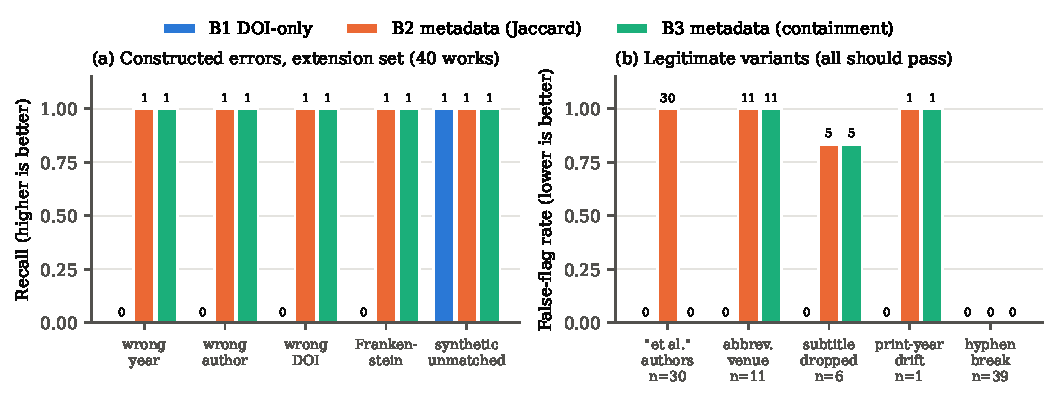
\includegraphics[width=\textwidth]{figures/fig_detection_false_flags.pdf}
\caption{(a) Recall per constructed error type on the extension set. (b) False-flag rate on legitimate variants of the same 40 works; numbers above the bars count false flags and $n$ is the number of cases. \BTwo{} and \BThree{} differ only on ``et al.'' author lists.}
\Description{Two grouped bar charts. Left: B1 has recall 0 on every error type except synthetic DOIs; B2 and B3 have recall 1 everywhere. Right: B2 false-flags all et-al, abbreviated-venue and print-year cases and 5 of 6 dropped subtitles; B3 differs only by passing all et-al cases; no method flags hyphen breaks.}
\label{fig:main}
\end{figure*}

\subsection{RQ2: where the checkers go wrong}
\paragraph{Misses.} \BOne{} misses wrong-year, wrong-author, wrong-DOI and Frankenstein citations without exception (recall 0 for each). A resolving DOI says that \emph{some} work exists at that address, and nothing about whether the citation describes it.

\paragraph{False flags on legitimate citations.} \BTwo{} flagged 47 of the 87 legitimate variants (54\%; bootstrap 0.50--0.58), against 0 for \BOne{}. That overall rate depends on the mix of variant types, which is set by applicability (39 hyphen breaks, which never fire, against one print-year case), so the per-type rates in Table~\ref{tab:stress} are the more meaningful numbers. Because \BTwo{} records which field failed, every false flag has one identifiable cause:
\begin{itemize}[leftmargin=1.2em,itemsep=1pt]
\item \emph{``et al.''} (30/30, author field). One cited name against $n$ real names gives a Jaccard of $1/n \leq 0.5$, which never reaches 0.80.
\item \emph{Abbreviated venue} (11/11, venue field). Exact matching can't equate ``Polym. Chem.''\ with ``Polymer Chemistry''. Some cases are also registry defects. Crossref stores one journal as ``Psychology \&amp; Marketing'', with an undecoded HTML entity, and another with a Unicode replacement character in place of ``ü''. Correct citations of these journals can never match exactly.
\item \emph{Subtitle dropped} (5/6, title field). Removing a long subtitle pushed title similarity down to 0.40--0.86. The one case that passed sat at 0.90.
\item \emph{Print-year drift} (1/1, year field). One article was published online in 2022 and in print in 2023. Citing the print year is normal practice, and \BTwo{} calls it an error.
\item \emph{Hyphen breaks} (0/39). Normalization plus a 0.90 similarity threshold absorbs them completely.
\end{itemize}

\begin{table}[t]
\caption{False flags on legitimate variants (extension set). All 87 cases are valid citations.}
\label{tab:stress}
\footnotesize
\begin{tabular*}{\linewidth}{@{\extracolsep{\fill}}lrrrrl@{}}
\toprule
Variant & $n$ & \BOne{} & \BTwo{} & \BThree{} & Field that fired \\
\midrule
``et al.''\ author list & 30 & 0 & 30 & 0 & authors \\
Abbreviated venue & 11 & 0 & 11 & 11 & venue \\
Subtitle dropped & 6 & 0 & 5 & 5 & title \\
Print-year drift & 1 & 0 & 1 & 1 & year \\
Hyphen break & 39 & 0 & 0 & 0 & -- \\
\midrule
Total (rate) & 87 & 0 (0.00) & 47 (0.54) & 17 (0.195) & \\
\bottomrule
\end{tabular*}
\end{table}

\paragraph{Field ablation.} Fig.~\ref{fig:ablation} places each ablated version of \BTwo{} by recall and false-flag rate. Two categories are caught by every variant: synthetic DOIs don't resolve, and a borrowed DOI leads to a different paper whose fields all disagree with the citation. Beyond that, each field earns exactly one category. Title catches Frankenstein citations, year catches wrong years and authors catch wrong authors. The venue check catches nothing the other three don't: removing it keeps macro recall at 1.00 and cuts false flags from 54\% to 41\%. I don't read this as ``venue checks are useless''. The design has no wrong-venue category, so the venue check had nothing to find. The fair conclusion is that, here, it cost 11 false flags and bought nothing.

\begin{figure}[t]
\centering
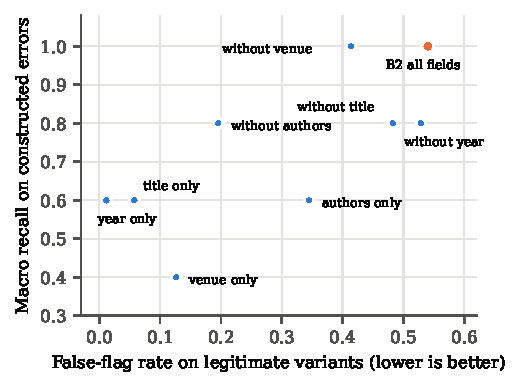
\includegraphics[width=0.62\linewidth]{figures/fig_ablation.pdf}
\caption{Field ablation of \BTwo{} on the extension set: macro recall on constructed errors against the false-flag rate on legitimate variants. Upper left is better.}
\Description{Scatter plot of nine B2 field variants. Full B2 sits at recall 1.0 and false-flag rate 0.54; removing venue keeps recall 1.0 at 0.41; single-field variants reach recall 0.4 to 0.6.}
\label{fig:ablation}
\end{figure}

\paragraph{Thresholds don't fix it.} Fig.~\ref{fig:sensitivity} shows that loosening the title threshold barely helps (54\% at 0.90, 51\% at 0.50). The dropped-subtitle cases sit below any sensible threshold, and the author and venue flags don't depend on it at all. A title threshold of 1.00 flags every hyphen-broken title. Loosening the author Jaccard threshold to 0.20 lowers false flags to 30\%, but ``et al.''\ citations of papers with long author lists still fail, because $1/17$ is below any threshold that would still catch a replaced author list. Recall stays at 1.00 across both sweeps, which again says more about the mutations than about robustness. The problem with the author check is the rule, not the cutoff.

\begin{figure*}[t]
\centering
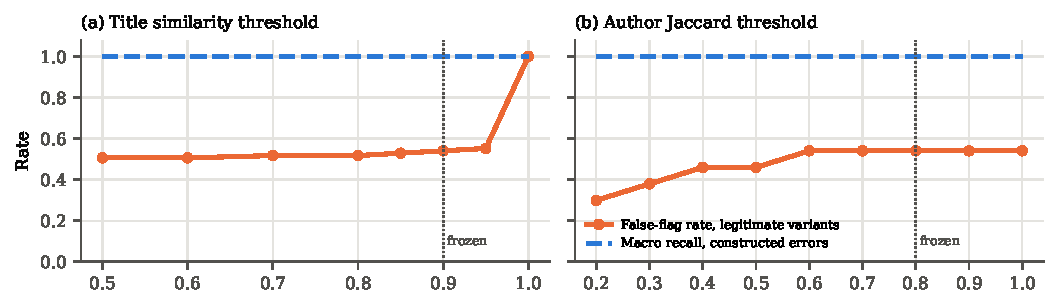
\includegraphics[width=\textwidth]{figures/fig_sensitivity.pdf}
\caption{Threshold sensitivity of \BTwo{} on the extension set. The dotted line marks the frozen operating point, which was not changed after these results were seen.}
\Description{Two line charts. Recall stays at 1.0 for all thresholds. False-flag rate stays near 0.5 for title thresholds 0.5 to 0.95 and jumps to 1.0 at 1.0; for author thresholds it falls from 0.54 to 0.30 as the threshold drops to 0.2.}
\label{fig:sensitivity}
\end{figure*}

\subsection{A single-rule change (\BThree{})}
Replacing the Jaccard rule with containment removed all 30 ``et al.''\ false flags and changed nothing else. The false-flag rate fell from 0.54 to 0.195 (paired bootstrap difference $-0.39$ to $-0.29$), and recall stayed at 1.00 in every error category, including wrong authors. \BThree{} reaches the same false-flag rate as dropping the author check entirely (Fig.~\ref{fig:ablation}, ``without authors'') but keeps the author check's recall. The hypothesis written down before the run is supported, but that result needs a caveat. The ``et al.''\ variant and the rule that fixes it were designed together in the same amendment, so removing those 30 flags demonstrates the mechanism. It doesn't validate containment as a better rule in general. The informative part is that no recall was lost, and even that is only weakly tested because no error category corrupts part of an author list. Its main blind spot is predictable: it would pass a citation that lists only a non-first co-author, which may or may not count as an error depending on the definition.

\subsection{RQ3: the definition moves the numbers}
Under identity-only labels (Table~\ref{tab:main}, last rows), a wrong year or a borrowed DOI is no longer an error. \BTwo{}'s predictions are unchanged, but its precision falls from 1.00 to 0.60 and its FPR rises from 0.00 to 0.40 on both held-out sets. \BOne{}'s recall rises from 0.20 to 0.33 only because there are fewer positives. The checkers didn't change at all. The same output looks like a perfect verifier under one definition and a noisy one under another. This is the same definitional problem that makes published fabrication rates hard to compare, and Russinovich et al.\ deliberately exclude venue and year drift from their count for this reason \citep{russinovich2026}.

\section{Discussion}
Taken together, the results describe a trade-off, not a winner. A DOI-only check is almost silent about false alarms and almost blind to errors in real citations. Field matching sees those errors, but at the frozen settings it called more than half of a sample of legitimate citations wrong. Every one of those false alarms has a mundane cause: citation conventions (``et al.'', abbreviated journals, short titles), publication-date ambiguity, and defects in the registry itself. A human reviewing \BTwo{}'s flags would spend most of their time dismissing them, which matches what Russinovich et al.\ report about their own tool \citep{russinovich2026}. This study puts a number on that effect for one simple design.

Two practical points follow. First, rules should encode citation semantics, not just string similarity. The containment rule is a one-line change that removed 64\% of the false flags here, because it reflects what a correct author list actually is. Venue matching would need the same treatment (registry short titles, entity decoding), and that change would have to be frozen before scoring, as \BThree{} was. Second, a checker's reported accuracy is only meaningful alongside its error definition and its tolerance for legitimate variation. The identity-only rescoring shows that the definition alone can move precision by 40 points.

\section{Limitations and Threats to Validity}
\begin{itemize}[leftmargin=1.2em,itemsep=1pt]
\item \emph{Constructed, not natural, errors.} Nothing here estimates how often language models fabricate citations, or how a checker would perform on real model output.
\item \emph{Shared registry.} Labels and lookups both come from Crossref, which makes recall on the error categories close to guaranteed. The legitimate-variant analysis reduces this circularity but doesn't remove it: those variants are still derived from registry fields.
\item \emph{Small samples.} Forty works is modest. Print-year drift ($n=1$) and dropped subtitles ($n=6$) are anecdotes, not rates. The test set of eight works came from a hand-picked list, which is why the random extension set was added.
\item \emph{Fix and test designed together.} \BThree{}'s rule and the ``et al.''\ variant were specified in the same amendment, so its improvement on that variant is by construction.\item \emph{Coverage of the design.} There is no wrong-venue or partial-author error category, so the ablation can't credit the venue check, and \BThree{}'s blind spots go untested. Only journal articles indexed by Crossref are included. Conference papers, books and preprints are not.
\item \emph{Abstention.} One in eight cases had no DOI, and none of these checkers can say anything about them. Real model output often lacks DOIs.
\item \emph{Simple checkers.} These are teaching controls. The findings say nothing direct about RefChecker, CiteCheck or any commercial tool.
\end{itemize}

\section{Conclusion}
A resolving DOI tells you that a work exists. It doesn't tell you that the citation describes it. In this controlled audit, a DOI-only control caught only non-existent DOIs, while field matching caught every constructed error but flagged more than half of a set of perfectly legitimate citations. Each false flag traced back to a single field rule, and changing one of those rules from a similarity threshold to a semantic containment check removed nearly two-thirds of the false flags without losing recall. The most useful next steps are cheap ones: add wrong-venue and partial-author error categories, test registry-aware venue normalization under a frozen protocol, and then score a small hand-labelled set of real model-generated references.

\section*{Reproducibility}
The repository contains the frozen protocol, the amendment (\texttt{contribution\_plan.md}), the Crossref fact cache, the snapshot and case files with their hashes, all scripts and tests, every prediction file and the logs. \texttt{python scripts/evaluate.py} followed by \texttt{python scripts/make\_figures.py} regenerates every table and figure offline from the cached data.

\section*{Use of AI Tools}
AI coding assistants were used throughout this project, and this is disclosed in detail in the repository's \texttt{ai\_assistance\_log.md} and \texttt{ai\_audit.md}. Claude Code (Claude Opus 5.5) was used in this phase to draft the amendment, implement and test the evaluation code, run the experiments, produce the figures and draft this manuscript. Earlier phases used other AI assistance, recorded in the same log. I checked the original source papers myself during the review phase, as recorded in the log. Every number in this paper comes from files generated by the released code. No result, citation or log was written by hand or invented. Every bibliography entry was checked against arXiv or Crossref.

\bibliographystyle{ACM-Reference-Format}
\bibliography{references}
\end{document}
